% Options for packages loaded elsewhere
\PassOptionsToPackage{unicode}{hyperref}
\PassOptionsToPackage{hyphens}{url}
%
\documentclass[
]{article}
\usepackage{amsmath,amssymb}
\usepackage{lmodern}
\usepackage{iftex}
\ifPDFTeX
  \usepackage[T1]{fontenc}
  \usepackage[utf8]{inputenc}
  \usepackage{textcomp} % provide euro and other symbols
\else % if luatex or xetex
  \usepackage{unicode-math}
  \defaultfontfeatures{Scale=MatchLowercase}
  \defaultfontfeatures[\rmfamily]{Ligatures=TeX,Scale=1}
\fi
% Use upquote if available, for straight quotes in verbatim environments
\IfFileExists{upquote.sty}{\usepackage{upquote}}{}
\IfFileExists{microtype.sty}{% use microtype if available
  \usepackage[]{microtype}
  \UseMicrotypeSet[protrusion]{basicmath} % disable protrusion for tt fonts
}{}
\makeatletter
\@ifundefined{KOMAClassName}{% if non-KOMA class
  \IfFileExists{parskip.sty}{%
    \usepackage{parskip}
  }{% else
    \setlength{\parindent}{0pt}
    \setlength{\parskip}{6pt plus 2pt minus 1pt}}
}{% if KOMA class
  \KOMAoptions{parskip=half}}
\makeatother
\usepackage{xcolor}
\usepackage[margin=1in]{geometry}
\usepackage{color}
\usepackage{fancyvrb}
\newcommand{\VerbBar}{|}
\newcommand{\VERB}{\Verb[commandchars=\\\{\}]}
\DefineVerbatimEnvironment{Highlighting}{Verbatim}{commandchars=\\\{\}}
% Add ',fontsize=\small' for more characters per line
\usepackage{framed}
\definecolor{shadecolor}{RGB}{248,248,248}
\newenvironment{Shaded}{\begin{snugshade}}{\end{snugshade}}
\newcommand{\AlertTok}[1]{\textcolor[rgb]{0.94,0.16,0.16}{#1}}
\newcommand{\AnnotationTok}[1]{\textcolor[rgb]{0.56,0.35,0.01}{\textbf{\textit{#1}}}}
\newcommand{\AttributeTok}[1]{\textcolor[rgb]{0.77,0.63,0.00}{#1}}
\newcommand{\BaseNTok}[1]{\textcolor[rgb]{0.00,0.00,0.81}{#1}}
\newcommand{\BuiltInTok}[1]{#1}
\newcommand{\CharTok}[1]{\textcolor[rgb]{0.31,0.60,0.02}{#1}}
\newcommand{\CommentTok}[1]{\textcolor[rgb]{0.56,0.35,0.01}{\textit{#1}}}
\newcommand{\CommentVarTok}[1]{\textcolor[rgb]{0.56,0.35,0.01}{\textbf{\textit{#1}}}}
\newcommand{\ConstantTok}[1]{\textcolor[rgb]{0.00,0.00,0.00}{#1}}
\newcommand{\ControlFlowTok}[1]{\textcolor[rgb]{0.13,0.29,0.53}{\textbf{#1}}}
\newcommand{\DataTypeTok}[1]{\textcolor[rgb]{0.13,0.29,0.53}{#1}}
\newcommand{\DecValTok}[1]{\textcolor[rgb]{0.00,0.00,0.81}{#1}}
\newcommand{\DocumentationTok}[1]{\textcolor[rgb]{0.56,0.35,0.01}{\textbf{\textit{#1}}}}
\newcommand{\ErrorTok}[1]{\textcolor[rgb]{0.64,0.00,0.00}{\textbf{#1}}}
\newcommand{\ExtensionTok}[1]{#1}
\newcommand{\FloatTok}[1]{\textcolor[rgb]{0.00,0.00,0.81}{#1}}
\newcommand{\FunctionTok}[1]{\textcolor[rgb]{0.00,0.00,0.00}{#1}}
\newcommand{\ImportTok}[1]{#1}
\newcommand{\InformationTok}[1]{\textcolor[rgb]{0.56,0.35,0.01}{\textbf{\textit{#1}}}}
\newcommand{\KeywordTok}[1]{\textcolor[rgb]{0.13,0.29,0.53}{\textbf{#1}}}
\newcommand{\NormalTok}[1]{#1}
\newcommand{\OperatorTok}[1]{\textcolor[rgb]{0.81,0.36,0.00}{\textbf{#1}}}
\newcommand{\OtherTok}[1]{\textcolor[rgb]{0.56,0.35,0.01}{#1}}
\newcommand{\PreprocessorTok}[1]{\textcolor[rgb]{0.56,0.35,0.01}{\textit{#1}}}
\newcommand{\RegionMarkerTok}[1]{#1}
\newcommand{\SpecialCharTok}[1]{\textcolor[rgb]{0.00,0.00,0.00}{#1}}
\newcommand{\SpecialStringTok}[1]{\textcolor[rgb]{0.31,0.60,0.02}{#1}}
\newcommand{\StringTok}[1]{\textcolor[rgb]{0.31,0.60,0.02}{#1}}
\newcommand{\VariableTok}[1]{\textcolor[rgb]{0.00,0.00,0.00}{#1}}
\newcommand{\VerbatimStringTok}[1]{\textcolor[rgb]{0.31,0.60,0.02}{#1}}
\newcommand{\WarningTok}[1]{\textcolor[rgb]{0.56,0.35,0.01}{\textbf{\textit{#1}}}}
\usepackage{graphicx}
\makeatletter
\def\maxwidth{\ifdim\Gin@nat@width>\linewidth\linewidth\else\Gin@nat@width\fi}
\def\maxheight{\ifdim\Gin@nat@height>\textheight\textheight\else\Gin@nat@height\fi}
\makeatother
% Scale images if necessary, so that they will not overflow the page
% margins by default, and it is still possible to overwrite the defaults
% using explicit options in \includegraphics[width, height, ...]{}
\setkeys{Gin}{width=\maxwidth,height=\maxheight,keepaspectratio}
% Set default figure placement to htbp
\makeatletter
\def\fps@figure{htbp}
\makeatother
\setlength{\emergencystretch}{3em} % prevent overfull lines
\providecommand{\tightlist}{%
  \setlength{\itemsep}{0pt}\setlength{\parskip}{0pt}}
\setcounter{secnumdepth}{-\maxdimen} % remove section numbering
\ifLuaTeX
  \usepackage{selnolig}  % disable illegal ligatures
\fi
\IfFileExists{bookmark.sty}{\usepackage{bookmark}}{\usepackage{hyperref}}
\IfFileExists{xurl.sty}{\usepackage{xurl}}{} % add URL line breaks if available
\urlstyle{same} % disable monospaced font for URLs
\hypersetup{
  pdftitle={My Jupyter Notebook Presentation},
  hidelinks,
  pdfcreator={LaTeX via pandoc}}

\title{My Jupyter Notebook Presentation}
\author{}
\date{\vspace{-2.5em}}

\begin{document}
\maketitle

\begin{Shaded}
\begin{Highlighting}[]
\ImportTok{import}\NormalTok{ numpy }\ImportTok{as}\NormalTok{ np}
\ImportTok{import}\NormalTok{ pandas }\ImportTok{as}\NormalTok{ pd}
\ImportTok{import}\NormalTok{ matplotlib.pyplot }\ImportTok{as}\NormalTok{ plt}
\ImportTok{import}\NormalTok{ plotly.express }\ImportTok{as}\NormalTok{ px}
\NormalTok{pd.options.plotting.backend}\OperatorTok{=} \StringTok{"plotly"}
\NormalTok{pd.set\_option(}\StringTok{\textquotesingle{}display.max\_columns\textquotesingle{}}\NormalTok{, }\DecValTok{150}\NormalTok{, }\StringTok{\textquotesingle{}display.max\_rows\textquotesingle{}}\NormalTok{, }\DecValTok{100}\NormalTok{, }\StringTok{\textquotesingle{}display.max\_colwidth\textquotesingle{}}\NormalTok{, }\DecValTok{15}\NormalTok{)}
\OperatorTok{\%}\NormalTok{matplotlib inline }
\end{Highlighting}
\end{Shaded}

\begin{Shaded}
\begin{Highlighting}[]
\CommentTok{\#!jupyter nbconvert {-}{-}to markdown {-}{-}output mymarkdownfile.md Anamoly\_detection\_credit\_card.ipynb}
\CommentTok{\#!pandoc mymarkdownfile.md {-}s {-}{-}mathml  {-}o mathMathML.html}
\CommentTok{\#!pandoc  mymarkdownfile.md  {-}t revealjs {-}V theme=white {-}V slideNumber=true {-}o index.html}
\end{Highlighting}
\end{Shaded}

\begin{Shaded}
\begin{Highlighting}[]

\CommentTok{\#!pandoc {-}t dzslides mymarkdown.md {-}o pandoc/dzslides{-}pandoc.html {-}{-}embed{-}resources {-}{-}standalone}
\CommentTok{\#!pandoc {-}t slidy habits.md {-}o pandoc/slidy{-}pandoc.html {-}{-}self{-}contained}
\CommentTok{\#!pandoc {-}t revealjs habits.md {-}o pandoc/revealjs{-}pandoc.html {-}sV revealjs{-}url=https://revealjs.com}
\CommentTok{\#!jupyter nbconvert {-}{-}to slides {-}{-}output mymarkdownfile.html Anamoly\_detection\_credit\_card.ipynb}
\CommentTok{\#!jupyter nbconvert {-}{-}to slides {-}{-}post serve Anamoly\_detection\_credit\_card.ipynb}
\CommentTok{\#!jupyter nbconvert {-}{-}to slides {-}{-}execute Anamoly\_detection\_credit\_card.ipynb}
\CommentTok{\#!pip install autoviz}
\end{Highlighting}
\end{Shaded}

\begin{itemize}
\item
  \protect\hyperlink{1}{Introduction}
\item
  \protect\hyperlink{2}{Methodology}
\item
  \protect\hyperlink{5}{Conclusion}
\end{itemize}

\# Introduction

\begin{itemize}
\item
  In the real world, fraud often goes undiscovered, and only the fraud
  that is caught provides any labels for the datasets.
\item
  Moreover, fraud patterns change over time, so supervised systems that
  are built using fraud labels become stale, capturing historical
  patterns of fraud but failing to adapt to newly emerging patterns.
\item
  For these reasons (the lack of sufficient labels and the need to adapt
  to newly emerging patterns of fraud as quickly as possible),
  unsupervised learning fraud detection systems are in vogue.
\item
  In this notebook, we will build such a solution using PCA
\end{itemize}

\hypertarget{what-is-pca}{%
\subsection{What is PCA}\label{what-is-pca}}

PCA (Principal Component Analysis) is a technique to find a
low-dimensional representation of a dataset that captures as much
variation as possible. It seeks a small number of dimensions that are
interesting and informative, where each dimension is a linear
combination of the original features. The first principal component is a
normalized linear combination of the features that has the largest
variance. It can be found through an optimization problem, and the
resulting loadings and scores make up the principal component loading
vector. PCA is useful when the original dataset has a large number of
features, making it difficult to visualize and analyze.

\begin{Shaded}
\begin{Highlighting}[]
\CommentTok{\# load dataset}
\NormalTok{df }\OperatorTok{=}\NormalTok{ pd.read\_csv(}\StringTok{\textquotesingle{}/Users/waleedidrees/Dropbox/Python\_Projects/books/handson{-}unsupervised{-}learning{-}master/datasets/credit\_card\_data/credit\_card.csv\textquotesingle{}}\NormalTok{).rename(columns}\OperatorTok{=}\NormalTok{ \{}\StringTok{"Class"}\NormalTok{:}\StringTok{"target"}\NormalTok{\})}
\NormalTok{df.head()}
\end{Highlighting}
\end{Shaded}

Time

V1

V2

V3

V4

V5

V6

V7

V8

V9

V10

V11

V12

V13

V14

V15

V16

V17

V18

V19

V20

V21

V22

V23

V24

V25

V26

V27

V28

Amount

target

0

0.0

-1.359807

-0.072781

2.536347

1.378155

-0.338321

0.462388

0.239599

0.098698

0.363787

0.090794

-0.551600

-0.617801

-0.991390

-0.311169

1.468177

-0.470401

0.207971

0.025791

0.403993

0.251412

-0.018307

0.277838

-0.110474

0.066928

0.128539

-0.189115

0.133558

-0.021053

149.62

0

1

0.0

1.191857

0.266151

0.166480

0.448154

0.060018

-0.082361

-0.078803

0.085102

-0.255425

-0.166974

1.612727

1.065235

0.489095

-0.143772

0.635558

0.463917

-0.114805

-0.183361

-0.145783

-0.069083

-0.225775

-0.638672

0.101288

-0.339846

0.167170

0.125895

-0.008983

0.014724

2.69

0

2

1.0

-1.358354

-1.340163

1.773209

0.379780

-0.503198

1.800499

0.791461

0.247676

-1.514654

0.207643

0.624501

0.066084

0.717293

-0.165946

2.345865

-2.890083

1.109969

-0.121359

-2.261857

0.524980

0.247998

0.771679

0.909412

-0.689281

-0.327642

-0.139097

-0.055353

-0.059752

378.66

0

3

1.0

-0.966272

-0.185226

1.792993

-0.863291

-0.010309

1.247203

0.237609

0.377436

-1.387024

-0.054952

-0.226487

0.178228

0.507757

-0.287924

-0.631418

-1.059647

-0.684093

1.965775

-1.232622

-0.208038

-0.108300

0.005274

-0.190321

-1.175575

0.647376

-0.221929

0.062723

0.061458

123.50

0

4

2.0

-1.158233

0.877737

1.548718

0.403034

-0.407193

0.095921

0.592941

-0.270533

0.817739

0.753074

-0.822843

0.538196

1.345852

-1.119670

0.175121

-0.451449

-0.237033

-0.038195

0.803487

0.408542

-0.009431

0.798278

-0.137458

0.141267

-0.206010

0.502292

0.219422

0.215153

69.99

0

\begin{Shaded}
\begin{Highlighting}[]
\NormalTok{df.columns}\OperatorTok{=}\NormalTok{ df.columns.}\BuiltInTok{str}\NormalTok{.lower()}
\NormalTok{df.head()}
\end{Highlighting}
\end{Shaded}

time

v1

v2

v3

v4

v5

v6

v7

v8

v9

v10

v11

v12

v13

v14

v15

v16

v17

v18

v19

v20

v21

v22

v23

v24

v25

v26

v27

v28

amount

target

0

0.0

-1.359807

-0.072781

2.536347

1.378155

-0.338321

0.462388

0.239599

0.098698

0.363787

0.090794

-0.551600

-0.617801

-0.991390

-0.311169

1.468177

-0.470401

0.207971

0.025791

0.403993

0.251412

-0.018307

0.277838

-0.110474

0.066928

0.128539

-0.189115

0.133558

-0.021053

149.62

0

1

0.0

1.191857

0.266151

0.166480

0.448154

0.060018

-0.082361

-0.078803

0.085102

-0.255425

-0.166974

1.612727

1.065235

0.489095

-0.143772

0.635558

0.463917

-0.114805

-0.183361

-0.145783

-0.069083

-0.225775

-0.638672

0.101288

-0.339846

0.167170

0.125895

-0.008983

0.014724

2.69

0

2

1.0

-1.358354

-1.340163

1.773209

0.379780

-0.503198

1.800499

0.791461

0.247676

-1.514654

0.207643

0.624501

0.066084

0.717293

-0.165946

2.345865

-2.890083

1.109969

-0.121359

-2.261857

0.524980

0.247998

0.771679

0.909412

-0.689281

-0.327642

-0.139097

-0.055353

-0.059752

378.66

0

3

1.0

-0.966272

-0.185226

1.792993

-0.863291

-0.010309

1.247203

0.237609

0.377436

-1.387024

-0.054952

-0.226487

0.178228

0.507757

-0.287924

-0.631418

-1.059647

-0.684093

1.965775

-1.232622

-0.208038

-0.108300

0.005274

-0.190321

-1.175575

0.647376

-0.221929

0.062723

0.061458

123.50

0

4

2.0

-1.158233

0.877737

1.548718

0.403034

-0.407193

0.095921

0.592941

-0.270533

0.817739

0.753074

-0.822843

0.538196

1.345852

-1.119670

0.175121

-0.451449

-0.237033

-0.038195

0.803487

0.408542

-0.009431

0.798278

-0.137458

0.141267

-0.206010

0.502292

0.219422

0.215153

69.99

0

\hypertarget{disable-the-warnings}{%
\section{Disable the warnings}\label{disable-the-warnings}}

\begin{Shaded}
\begin{Highlighting}[]
\ImportTok{import}\NormalTok{ warnings}
\NormalTok{warnings.filterwarnings(}\StringTok{\textquotesingle{}ignore\textquotesingle{}}\NormalTok{)}
\end{Highlighting}
\end{Shaded}

\begin{Shaded}
\begin{Highlighting}[]
\NormalTok{df.describe().T}
\end{Highlighting}
\end{Shaded}

count

mean

std

min

25\%

50\%

75\%

max

time

284807.0

9.481386e+04

47488.145955

0.000000

54201.500000

84692.000000

139320.500000

172792.000000

v1

284807.0

1.168375e-15

1.958696

-56.407510

-0.920373

0.018109

1.315642

2.454930

v2

284807.0

3.416908e-16

1.651309

-72.715728

-0.598550

0.065486

0.803724

22.057729

v3

284807.0

-1.379537e-15

1.516255

-48.325589

-0.890365

0.179846

1.027196

9.382558

v4

284807.0

2.074095e-15

1.415869

-5.683171

-0.848640

-0.019847

0.743341

16.875344

v5

284807.0

9.604066e-16

1.380247

-113.743307

-0.691597

-0.054336

0.611926

34.801666

v6

284807.0

1.487313e-15

1.332271

-26.160506

-0.768296

-0.274187

0.398565

73.301626

v7

284807.0

-5.556467e-16

1.237094

-43.557242

-0.554076

0.040103

0.570436

120.589494

v8

284807.0

1.213481e-16

1.194353

-73.216718

-0.208630

0.022358

0.327346

20.007208

v9

284807.0

-2.406331e-15

1.098632

-13.434066

-0.643098

-0.051429

0.597139

15.594995

v10

284807.0

2.239053e-15

1.088850

-24.588262

-0.535426

-0.092917

0.453923

23.745136

v11

284807.0

1.673327e-15

1.020713

-4.797473

-0.762494

-0.032757

0.739593

12.018913

v12

284807.0

-1.247012e-15

0.999201

-18.683715

-0.405571

0.140033

0.618238

7.848392

v13

284807.0

8.190001e-16

0.995274

-5.791881

-0.648539

-0.013568

0.662505

7.126883

v14

284807.0

1.207294e-15

0.958596

-19.214325

-0.425574

0.050601

0.493150

10.526766

v15

284807.0

4.887456e-15

0.915316

-4.498945

-0.582884

0.048072

0.648821

8.877742

v16

284807.0

1.437716e-15

0.876253

-14.129855

-0.468037

0.066413

0.523296

17.315112

v17

284807.0

-3.772171e-16

0.849337

-25.162799

-0.483748

-0.065676

0.399675

9.253526

v18

284807.0

9.564149e-16

0.838176

-9.498746

-0.498850

-0.003636

0.500807

5.041069

v19

284807.0

1.039917e-15

0.814041

-7.213527

-0.456299

0.003735

0.458949

5.591971

v20

284807.0

6.406204e-16

0.770925

-54.497720

-0.211721

-0.062481

0.133041

39.420904

v21

284807.0

1.654067e-16

0.734524

-34.830382

-0.228395

-0.029450

0.186377

27.202839

v22

284807.0

-3.568593e-16

0.725702

-10.933144

-0.542350

0.006782

0.528554

10.503090

v23

284807.0

2.578648e-16

0.624460

-44.807735

-0.161846

-0.011193

0.147642

22.528412

v24

284807.0

4.473266e-15

0.605647

-2.836627

-0.354586

0.040976

0.439527

4.584549

v25

284807.0

5.340915e-16

0.521278

-10.295397

-0.317145

0.016594

0.350716

7.519589

v26

284807.0

1.683437e-15

0.482227

-2.604551

-0.326984

-0.052139

0.240952

3.517346

v27

284807.0

-3.660091e-16

0.403632

-22.565679

-0.070840

0.001342

0.091045

31.612198

v28

284807.0

-1.227390e-16

0.330083

-15.430084

-0.052960

0.011244

0.078280

33.847808

amount

284807.0

8.834962e+01

250.120109

0.000000

5.600000

22.000000

77.165000

25691.160000

target

284807.0

1.727486e-03

0.041527

0.000000

0.000000

0.000000

0.000000

1.000000

\hypertarget{we-see-that-fraudulent-transactions-are-very-rare-and-this-makes-the-data-very-imbalanced}{%
\subsection{we see that fraudulent transactions are very rare and this
makes the data very
imbalanced}\label{we-see-that-fraudulent-transactions-are-very-rare-and-this-makes-the-data-very-imbalanced}}

\begin{Shaded}
\begin{Highlighting}[]
\NormalTok{df[}\StringTok{"target"}\NormalTok{].value\_counts().reset\_index()}
\end{Highlighting}
\end{Shaded}

index

target

0

0

284315

1

1

492

we have 284,807 credit card transactions in total, of which 492 are
fraudulent, with a positive (fraud) label of one. The rest are normal
transactions, with a negative (not fraud) label of zero. We have 30
features to use for anomaly detection---time, amount, and 28 principal
components. And, we will split the dataset into a training set (with
190,820 transactions and 330 cases of fraud) and a test set (with the
remaining 93,987 transactions and 162 cases of fraud)

\begin{Shaded}
\begin{Highlighting}[]
\NormalTok{(}
\NormalTok{df[}\StringTok{"target"}\NormalTok{]}
\NormalTok{.value\_counts()}
\NormalTok{.reset\_index()}
\NormalTok{.plot.bar(x}\OperatorTok{=}\StringTok{"index"}\NormalTok{, y}\OperatorTok{=} \StringTok{"target"}\NormalTok{, color}\OperatorTok{=}\StringTok{"index"}\NormalTok{, height}\OperatorTok{=} \DecValTok{800}\NormalTok{, width}\OperatorTok{=} \DecValTok{800}\NormalTok{)}
\NormalTok{ )}
\end{Highlighting}
\end{Shaded}

\begin{Shaded}
\begin{Highlighting}[]
\NormalTok{pd.options.plotting.backend }\OperatorTok{=} \StringTok{"matplotlib"}

\NormalTok{df.hist(figsize}\OperatorTok{=}\NormalTok{ (}\DecValTok{22}\NormalTok{,}\DecValTok{16}\NormalTok{), bins}\OperatorTok{=}\DecValTok{50}\NormalTok{)}

\NormalTok{pd.options.plotting.backend }\OperatorTok{=} \StringTok{"plotly"}
\end{Highlighting}
\end{Shaded}

\begin{figure}
\centering
\includegraphics{mymarkdownfile_files/mymarkdownfile_15_0.png}
\caption{png}
\end{figure}

\hypertarget{methodology}{%
\subsection{Methodology}\label{methodology}}

Since this an unsupervised learning problem and we will not be using the
labels so we need find a way to measure the performance of the anamoly
model. Dimensionality reduction algorithms reduce the dimensionality of
data while attempting to minimize the reconstruction error. However,
these dimensionality reduction algorithms cannot capture all the
information of the original features as they move to a lower dimensional
space; therefore, there will be some error as these algorithms
reconstruct the reduced feature set back to the original number of
dimensions. we will use these errors and make a function to compare them
to the original dataframe and measure the score. we make our performance
measure as follows:

\begin{itemize}
\tightlist
\item
  We take the difference between the original vs the pca dataframe which
  we created from pcs components using inverse transformation
\item
  then we transform the difference using min max scaller from 0 to 1
  scale
\item
  we can consider this score as probability score and use this against
  the labels to calculate, precision, recall and threshhold using
  sklearn precision recall curve metric.
\item
  We will take x number of highest scores as our anomolies
\item
  we can all also calculate average precision score using the average
  precision score metric.
\end{itemize}

\hypertarget{define-evaluation-functions}{%
\section{Define evaluation
functions}\label{define-evaluation-functions}}

\begin{Shaded}
\begin{Highlighting}[]
\CommentTok{\# Calculate reconstruction error}
\KeywordTok{def}\NormalTok{ anomalyScores(originalDF, pca\_df):}
\NormalTok{    loss }\OperatorTok{=}\NormalTok{ ((originalDF.values}\OperatorTok{{-}}\NormalTok{ pca\_df.values)}\OperatorTok{**}\DecValTok{2}\NormalTok{).}\BuiltInTok{sum}\NormalTok{(axis}\OperatorTok{=}\DecValTok{1}\NormalTok{)    }
\NormalTok{    loss }\OperatorTok{=}\NormalTok{ pd.Series(data}\OperatorTok{=}\NormalTok{loss,index}\OperatorTok{=}\NormalTok{originalDF.index)}
\NormalTok{    loss }\OperatorTok{=}\NormalTok{ (loss}\OperatorTok{{-}}\NormalTok{np.}\BuiltInTok{min}\NormalTok{(loss))}\OperatorTok{/}\NormalTok{(np.}\BuiltInTok{max}\NormalTok{(loss)}\OperatorTok{{-}}\NormalTok{np.}\BuiltInTok{min}\NormalTok{(loss))}
    \ControlFlowTok{return}\NormalTok{ loss}
\end{Highlighting}
\end{Shaded}

\hypertarget{train-test-splits}{%
\section{Train-test splits}\label{train-test-splits}}

We will remove the target variable and we will not be using it for
training but we will use it to evaluate the anamolies by attaching it to
anamoly scores

\begin{Shaded}
\begin{Highlighting}[]
\ImportTok{from}\NormalTok{ sklearn.model\_selection }\ImportTok{import}\NormalTok{ train\_test\_split}
\NormalTok{X\_train, X\_test, y\_train, y\_test }\OperatorTok{=}\NormalTok{  train\_test\_split(df.drop(columns}\OperatorTok{=}\NormalTok{[}\StringTok{"target"}\NormalTok{,}\StringTok{"time"}\NormalTok{]).copy(), df[}\StringTok{"target"}\NormalTok{], test\_size }\OperatorTok{=} \FloatTok{0.33}\NormalTok{,stratify}\OperatorTok{=}\NormalTok{df[}\StringTok{"target"}\NormalTok{],  random\_state }\OperatorTok{=} \DecValTok{2018}\NormalTok{ )}
\NormalTok{X\_train.shape, y\_train.shape, X\_test.shape, y\_test.shape}
\end{Highlighting}
\end{Shaded}

\begin{verbatim}
((190820, 29), (190820,), (93987, 29), (93987,))
\end{verbatim}

The train data has 330 Fraudulent transaction and 190490 normal
transactions

\begin{Shaded}
\begin{Highlighting}[]
\NormalTok{y\_train.value\_counts()}
\end{Highlighting}
\end{Shaded}

\begin{verbatim}
0    190490
1       330
Name: target, dtype: int64
\end{verbatim}

\hypertarget{lets-create-preprocessing-pipiline}{%
\section{Lets create Preprocessing
Pipiline}\label{lets-create-preprocessing-pipiline}}

\begin{itemize}
\tightlist
\item
  all our variables are numeric we will standardise data and then as for
  PCA we must standardise observations.
\end{itemize}

\begin{Shaded}
\begin{Highlighting}[]
\ImportTok{from}\NormalTok{ sklearn.preprocessing }\ImportTok{import}\NormalTok{ StandardScaler}
\ImportTok{from}\NormalTok{ sklearn.pipeline }\ImportTok{import}\NormalTok{ Pipeline}
\ImportTok{from}\NormalTok{ sklearn.compose }\ImportTok{import}\NormalTok{ ColumnTransformer}
\ImportTok{from}\NormalTok{ sklearn.decomposition }\ImportTok{import}\NormalTok{ PCA}
\ImportTok{from}\NormalTok{ sklearn.impute }\ImportTok{import}\NormalTok{ KNNImputer}
\end{Highlighting}
\end{Shaded}

\begin{Shaded}
\begin{Highlighting}[]
\NormalTok{num\_pipe}\OperatorTok{=}\NormalTok{ Pipeline ( steps}\OperatorTok{=}\NormalTok{[}
\NormalTok{    (}\StringTok{"std"}\NormalTok{, StandardScaler()),}
\NormalTok{    (}\StringTok{"impute"}\NormalTok{, KNNImputer()), }
\NormalTok{    ])}
\end{Highlighting}
\end{Shaded}

\begin{Shaded}
\begin{Highlighting}[]
\NormalTok{all\_cols}\OperatorTok{=}\NormalTok{ X\_train.columns}
\NormalTok{prep}\OperatorTok{=}\NormalTok{ ColumnTransformer([}
\NormalTok{    (}\StringTok{"n"}\NormalTok{, num\_pipe, all\_cols)}
\NormalTok{    ]).set\_output(transform}\OperatorTok{=} \StringTok{"pandas"}\NormalTok{)}
\NormalTok{prep.fit\_transform(X\_train).head()}
\end{Highlighting}
\end{Shaded}

n\_\_v1

n\_\_v2

n\_\_v3

n\_\_v4

n\_\_v5

n\_\_v6

n\_\_v7

n\_\_v8

n\_\_v9

n\_\_v10

n\_\_v11

n\_\_v12

n\_\_v13

n\_\_v14

n\_\_v15

n\_\_v16

n\_\_v17

n\_\_v18

n\_\_v19

n\_\_v20

n\_\_v21

n\_\_v22

n\_\_v23

n\_\_v24

n\_\_v25

n\_\_v26

n\_\_v27

n\_\_v28

n\_\_amount

142087

-1.008613

1.168013

0.203077

-0.252933

-0.387030

-0.051340

-0.191393

0.917626

-0.220348

0.379391

0.891953

0.652099

-0.481673

0.888920

0.511094

0.459652

-0.178769

-0.131099

-0.030699

0.240351

-0.230649

-0.781406

0.154163

-0.584578

-0.161870

0.232116

0.525621

0.459397

-0.301324

165168

0.071848

0.664025

-0.240845

-0.381091

0.694608

-0.633906

0.833474

-0.132701

-0.166967

-0.793682

-0.490992

0.366808

0.879055

-1.245368

-0.369767

0.316392

0.393419

-0.407275

-0.310150

0.099453

-0.438520

-1.037593

0.145573

1.078771

-0.761303

0.221753

0.564899

0.254973

-0.342346

235908

0.099163

-0.387383

-0.945009

-1.493663

-0.092322

-0.878326

1.252531

-0.564372

-2.760963

0.979945

-0.734286

-0.940293

0.749094

0.176712

-1.084605

-2.049873

1.119388

-0.424709

0.039325

0.136822

0.597949

2.047828

0.533608

1.885871

-0.949325

0.195840

0.394576

0.789716

0.507010

148255

0.015486

0.519611

0.193472

-0.418969

0.316777

-0.774851

0.816615

-0.154107

-0.060485

-0.393037

-0.838072

0.229399

0.138905

0.095691

-0.404080

-0.180757

-0.428453

-1.022053

-0.193808

-0.038190

-0.336778

-0.738483

0.127711

-0.026519

-0.955999

0.297594

0.620507

0.285961

-0.333753

145672

0.009053

0.524138

0.175338

-0.335413

0.761346

0.501074

0.266188

0.187765

-0.186259

-0.837330

0.231244

0.693028

1.261985

-1.542311

-0.324732

1.234117

-0.316896

1.377317

0.854111

0.109213

-0.199423

-0.454902

0.047231

-0.725277

-2.181428

-0.147735

0.586351

0.739459

-0.337806

\hypertarget{pca-custom-class}{%
\subsection{PCA custom class}\label{pca-custom-class}}

\begin{itemize}
\tightlist
\item
  We create a Custom Transformer which will give us labels on the basis
  of top 350 highest anomoly score using our performace score function
\item
  this will be added in predict method.
\end{itemize}

\begin{Shaded}
\begin{Highlighting}[]
\ImportTok{from}\NormalTok{ sklearn.base }\ImportTok{import}\NormalTok{ MetaEstimatorMixin, clone}
\ImportTok{from}\NormalTok{ sklearn.base }\ImportTok{import}\NormalTok{ BaseEstimator, TransformerMixin}

\KeywordTok{class}\NormalTok{ pca\_anom(BaseEstimator, TransformerMixin):}
    \KeywordTok{def} \FunctionTok{\_\_init\_\_}\NormalTok{(}\VariableTok{self}\NormalTok{,estimator, top\_x):           }
        \VariableTok{self}\NormalTok{.estimator }\OperatorTok{=}\NormalTok{ estimator}
        \VariableTok{self}\NormalTok{.top\_x }\OperatorTok{=}\NormalTok{top\_x}
    
    \KeywordTok{def}\NormalTok{ fit(}\VariableTok{self}\NormalTok{, X,y}\OperatorTok{=}\VariableTok{None}\NormalTok{):       }
\NormalTok{       estimator\_}\OperatorTok{=}\NormalTok{ clone(}\VariableTok{self}\NormalTok{.estimator)}
       \VariableTok{self}\NormalTok{.model}\OperatorTok{=}\NormalTok{ estimator\_.fit(X)}
       \ControlFlowTok{return} \VariableTok{self}   
        
    \KeywordTok{def}\NormalTok{ transform(}\VariableTok{self}\NormalTok{, X, y}\OperatorTok{=}\VariableTok{None}\NormalTok{):                }
        \VariableTok{self}\NormalTok{.columns }\OperatorTok{=} \VariableTok{self}\NormalTok{.model.transform(X).shape[}\DecValTok{1}\NormalTok{]        }
        \ControlFlowTok{return} \VariableTok{self}\NormalTok{.model.transform(X)}
    
    \KeywordTok{def}\NormalTok{ get\_feature\_names\_out(}\VariableTok{self}\NormalTok{, names}\OperatorTok{=}\VariableTok{None}\NormalTok{):        }
        \ControlFlowTok{return}\NormalTok{ [}\SpecialStringTok{f\textquotesingle{}pca}\SpecialCharTok{\{}\NormalTok{x}\SpecialCharTok{\}}\SpecialStringTok{\textquotesingle{}}\ControlFlowTok{for}\NormalTok{ x }\KeywordTok{in} \BuiltInTok{range}\NormalTok{(}\VariableTok{self}\NormalTok{.columns) ]    }
    
    \KeywordTok{def}\NormalTok{ predict(}\VariableTok{self}\NormalTok{, X ):                   }
\NormalTok{        df\_pca\_inv}\OperatorTok{=}\NormalTok{ pd.DataFrame(}\VariableTok{self}\NormalTok{.model.inverse\_transform(}\VariableTok{self}\NormalTok{.model.transform(X)))}
\NormalTok{        df\_pca\_inv.columns}\OperatorTok{=}\NormalTok{ X.columns       }
\NormalTok{        results}\OperatorTok{=}\NormalTok{ pd.DataFrame()        }
\NormalTok{        results[}\StringTok{"prob"}\NormalTok{]}\OperatorTok{=}\NormalTok{ anomalyScores(X,df\_pca\_inv)}
\NormalTok{        anamloies}\OperatorTok{=}\NormalTok{ results.sort\_values(}\StringTok{"prob"}\NormalTok{ , ascending}\OperatorTok{=} \VariableTok{False}\NormalTok{).head(}\VariableTok{self}\NormalTok{.top\_x)        }
\NormalTok{        results}\OperatorTok{=}\NormalTok{ results.assign(class\_}\OperatorTok{=}\NormalTok{  np.where(results.index.isin(anamloies.index), }\DecValTok{1}\NormalTok{,}\DecValTok{0}\NormalTok{ ))}
        \ControlFlowTok{return}\NormalTok{ results[[}\StringTok{"class\_"}\NormalTok{]]}
    
    \KeywordTok{def}\NormalTok{ predict\_proba(}\VariableTok{self}\NormalTok{, X ):             }
\NormalTok{        df\_pca\_inv}\OperatorTok{=}\NormalTok{ pd.DataFrame(}\VariableTok{self}\NormalTok{.model.inverse\_transform(}\VariableTok{self}\NormalTok{.model.transform(X)))}
\NormalTok{        df\_pca\_inv.columns}\OperatorTok{=}\NormalTok{ X.columns       }
\NormalTok{        results}\OperatorTok{=}\NormalTok{ pd.DataFrame()        }
\NormalTok{        results[}\StringTok{"prob"}\NormalTok{]}\OperatorTok{=}\NormalTok{ anomalyScores(X,df\_pca\_inv)}
        \ControlFlowTok{return}\NormalTok{ results}
\end{Highlighting}
\end{Shaded}

\hypertarget{lets-define-evaluation-function-to-measure-the-recall-precision-and-roc_auc-score}{%
\section{Lets define Evaluation Function to measure the recall,
precision and roc\_auc
score}\label{lets-define-evaluation-function-to-measure-the-recall-precision-and-roc_auc-score}}

\begin{Shaded}
\begin{Highlighting}[]
\CommentTok{\# Evaluation Functions}
\ImportTok{from}\NormalTok{ sklearn.metrics }\ImportTok{import}\NormalTok{ accuracy\_score, recall\_score ,average\_precision\_score, precision\_recall\_curve, precision\_score, roc\_auc\_score,roc\_curve, auc }
\KeywordTok{def}\NormalTok{ eval\_scores(actuals, pred):}
\NormalTok{    res}\OperatorTok{=}\NormalTok{ pd.DataFrame(\{ }
    \StringTok{"accuracy"}\NormalTok{: [accuracy\_score(actuals, pred)], }
    \StringTok{"recall"}\NormalTok{: [recall\_score(actuals, pred)],}
    \StringTok{"roc\_auc"}\NormalTok{: [roc\_auc\_score(actuals, pred)],}
    \StringTok{"precision"}\NormalTok{: [precision\_score(actuals, pred)]\})    }
    \ControlFlowTok{return}\NormalTok{ res}
\end{Highlighting}
\end{Shaded}

\hypertarget{define-our-pca-model-pipeline-and-see-if-it-works-fine-with-custom-transformer}{%
\section{Define our PCA model pipeline and see if it works fine with
custom
Transformer}\label{define-our-pca-model-pipeline-and-see-if-it-works-fine-with-custom-transformer}}

\begin{Shaded}
\begin{Highlighting}[]
\ImportTok{from}\NormalTok{ sklearn.decomposition }\ImportTok{import}\NormalTok{ FastICA}
\NormalTok{pipe}\OperatorTok{=}\NormalTok{ Pipeline(steps}\OperatorTok{=}\NormalTok{[}
\NormalTok{    (}\StringTok{"preprocess"}\NormalTok{, prep),    }
\NormalTok{    (}\StringTok{\textquotesingle{}model\textquotesingle{}}\NormalTok{, pca\_anom(PCA(n\_components}\OperatorTok{=} \DecValTok{29}\NormalTok{, random\_state}\OperatorTok{=}\DecValTok{2018}\NormalTok{), top\_x}\OperatorTok{=}\DecValTok{350}\NormalTok{))        }
\NormalTok{    ]).set\_output(transform}\OperatorTok{=}\StringTok{"pandas"}\NormalTok{)}

\NormalTok{pipe.fit(X\_train,y\_train)}
\end{Highlighting}
\end{Shaded}

\hypertarget{sk-container-id-1}{}
In a Jupyter environment, please rerun this cell to show the HTML
representation or trust the notebook. On GitHub, the HTML representation
is unable to render, please try loading this page with nbviewer.org.

Pipeline

preprocess: ColumnTransformer

n

StandardScaler

KNNImputer

model: pca\_anom

estimator: PCA

PCA

\begin{Shaded}
\begin{Highlighting}[]
\NormalTok{pipe.fit\_transform(X\_train,y\_train).head()}
\end{Highlighting}
\end{Shaded}

pca0

pca1

pca2

pca3

pca4

pca5

pca6

pca7

pca8

pca9

pca10

pca11

pca12

pca13

pca14

pca15

pca16

pca17

pca18

pca19

pca20

pca21

pca22

pca23

pca24

pca25

pca26

pca27

pca28

142087

-0.503552

-0.086557

0.078180

0.126792

-0.584275

0.205438

-0.338339

0.301065

0.277474

-0.326303

0.129312

0.625587

-0.589936

1.110826

-0.613716

0.206283

0.647110

0.469355

-0.617997

-0.035442

-0.274916

0.403849

-1.131572

0.534247

0.506733

0.491447

-1.164396

-0.262446

-0.082420

165168

-0.445917

-0.295530

-0.008904

0.328010

0.591009

0.274222

1.074437

0.179167

0.291048

0.884476

-0.755596

-0.313761

-0.770876

-1.111460

-0.231645

-0.408441

-1.469363

0.413926

-0.430565

-0.612094

0.312883

-0.148244

-0.611249

-0.136882

-0.126312

0.857455

-0.303929

-0.105879

0.042523

235908

0.896149

-0.289270

-0.568506

-0.213853

0.772360

-0.916064

-0.826229

-1.543692

-0.180750

1.543498

-2.307194

0.847058

-0.623454

-1.268817

-0.570688

2.311289

-1.469729

0.404492

0.542410

1.540824

-0.153559

0.139862

1.148263

-1.707982

-1.496720

-0.135309

-0.550657

-0.127613

0.150344

148255

-0.418133

-0.359931

-0.092716

0.091789

-0.325522

0.539763

-0.005340

0.631961

0.437864

0.188399

-0.523586

-0.853044

-0.115711

-0.720514

-0.651368

0.436623

-0.990073

0.117838

-0.525740

0.082468

0.317526

0.196801

-0.800332

-0.439747

-0.188850

0.800011

-0.290804

-0.164921

0.053739

145672

-0.452670

-0.122389

0.055489

0.482373

0.428815

0.453595

1.774697

0.222596

-0.215380

1.321750

-0.540286

-0.297360

0.915669

1.534018

-0.618697

-1.442722

-1.529420

0.225133

-0.524002

-0.002704

-0.005569

-1.152543

-0.617781

-0.312699

0.493600

0.346001

-0.893674

-0.111020

0.052034

\hypertarget{seems-like-its-working-as-intended}{%
\subsection{Seems like its working as
intended}\label{seems-like-its-working-as-intended}}

\begin{itemize}
\tightlist
\item
  If we use PCA to generate the same number of principal components as
  the number of original features, will we wont be able to detect
  anamolies successfuly. When the number of principal components equals
  the number of original dimensions, PCA captures nearly 100\% of the
  variance/information in the data as it generates the principal
  components, and will have very little error. We will not be able to
  differentiate between rare transactions and normal ones---in other
  words, anomaly detection will be poor.
\item
  so lets run PCA for 20 to 30 components and see what number gives us
  best performance.
\end{itemize}

\begin{Shaded}
\begin{Highlighting}[]
\NormalTok{models}\OperatorTok{=}\NormalTok{ \{\}}
\NormalTok{scores}\OperatorTok{=}\NormalTok{ \{\}}
\ControlFlowTok{for}\NormalTok{ j }\KeywordTok{in} \BuiltInTok{range}\NormalTok{(}\DecValTok{20}\NormalTok{,}\DecValTok{30}\NormalTok{):}
\NormalTok{    models[}\StringTok{"pca"}\OperatorTok{+}\BuiltInTok{str}\NormalTok{(j)]}\OperatorTok{=}\NormalTok{ pipe.set\_params(}\OperatorTok{**}\NormalTok{\{}\StringTok{"model\_\_estimator\_\_n\_components"}\NormalTok{: j \})}
\NormalTok{    models[}\StringTok{"pca"}\OperatorTok{+}\BuiltInTok{str}\NormalTok{(j)].fit(X\_train)}
\NormalTok{    scores[}\StringTok{"pca"}\OperatorTok{+}\BuiltInTok{str}\NormalTok{(j)]}\OperatorTok{=}\NormalTok{ eval\_scores(y\_train, models[}\StringTok{"pca"}\OperatorTok{+}\BuiltInTok{str}\NormalTok{(j)].predict(X\_train) )}
\end{Highlighting}
\end{Shaded}

\begin{Shaded}
\begin{Highlighting}[]
\NormalTok{pd.concat(scores).sort\_values(}\StringTok{"recall"}\NormalTok{, ascending}\OperatorTok{=}\VariableTok{False}\NormalTok{) }
\end{Highlighting}
\end{Shaded}

accuracy

recall

roc\_auc

precision

pca27

0

0.999182

0.793939

0.896739

0.748571

pca26

0

0.998292

0.536364

0.767728

0.505714

pca25

0

0.998176

0.503030

0.751032

0.474286

pca23

0

0.997809

0.396970

0.697910

0.374286

pca24

0

0.997778

0.387879

0.693357

0.365714

pca22

0

0.997757

0.381818

0.690321

0.360000

pca21

0

0.997736

0.375758

0.687286

0.354286

pca20

0

0.997684

0.360606

0.679697

0.340000

pca29

0

0.997160

0.209091

0.603808

0.197143

pca28

0

0.996457

0.006061

0.502117

0.005714

\begin{itemize}
\tightlist
\item
  we can see from the Score above that 27 PCA components are the
  solution for this model and the Recall is .79 and precision is .75
  with roc\_auc of almost 0.9.
\end{itemize}

\begin{Shaded}
\begin{Highlighting}[]
\NormalTok{pipe.set\_params(}\OperatorTok{**}\NormalTok{\{}\StringTok{"model\_\_estimator\_\_n\_components"}\NormalTok{: }\DecValTok{27}\NormalTok{\})}
\NormalTok{pipe.fit(X\_train)}
\NormalTok{eval\_scores(y\_train, pipe.predict(X\_train) )}
\end{Highlighting}
\end{Shaded}

accuracy

recall

roc\_auc

precision

0

0.999182

0.793939

0.896739

0.748571

\begin{Shaded}
\begin{Highlighting}[]
\ImportTok{from}\NormalTok{ sklearn.metrics }\ImportTok{import}\NormalTok{ confusion\_matrix, ConfusionMatrixDisplay}
\NormalTok{cm }\OperatorTok{=}\NormalTok{ confusion\_matrix(y\_train, pipe.predict(X\_train), labels}\OperatorTok{=}\NormalTok{ y\_train.unique())}
\NormalTok{disp }\OperatorTok{=}\NormalTok{ ConfusionMatrixDisplay(confusion\_matrix}\OperatorTok{=}\NormalTok{cm,display\_labels}\OperatorTok{=}\NormalTok{ y\_train.unique())}
\NormalTok{disp.plot()}
\NormalTok{plt.show()}
\end{Highlighting}
\end{Shaded}

\begin{figure}
\centering
\includegraphics{mymarkdownfile_files/mymarkdownfile_40_0.png}
\caption{png}
\end{figure}

\begin{itemize}
\tightlist
\item
  This results is impressive considering its a unsupervised model we
  managed to etect 261 out of 330 fraudulent transactions.
\end{itemize}

\begin{Shaded}
\begin{Highlighting}[]
\NormalTok{preds}\OperatorTok{=}\NormalTok{ pd.concat([y\_train, pipe.predict\_proba(X\_train)], axis}\OperatorTok{=}\DecValTok{1}\NormalTok{)}
\NormalTok{preds.columns }\OperatorTok{=}\NormalTok{ [}\StringTok{\textquotesingle{}trueLabel\textquotesingle{}}\NormalTok{, }\StringTok{\textquotesingle{}anomalyScore\textquotesingle{}}\NormalTok{]}
\NormalTok{preds}
\end{Highlighting}
\end{Shaded}

trueLabel

anomalyScore

142087

0

3.343304e-05

165168

0

5.751799e-06

235908

0

1.718168e-05

148255

0

1.329301e-05

145672

0

6.641812e-06

\ldots{}

\ldots{}

\ldots{}

30023

0

1.068002e-07

195475

0

3.632382e-05

48687

0

1.021965e-05

159608

0

2.112043e-05

197673

0

3.677641e-05

190820 rows × 2 columns

\begin{Shaded}
\begin{Highlighting}[]
\NormalTok{precision, recall, thresholds }\OperatorTok{=}\NormalTok{  precision\_recall\_curve(preds[}\StringTok{\textquotesingle{}trueLabel\textquotesingle{}}\NormalTok{],preds[}\StringTok{\textquotesingle{}anomalyScore\textquotesingle{}}\NormalTok{])}
\NormalTok{average\_precision }\OperatorTok{=}\NormalTok{  average\_precision\_score(preds[}\StringTok{\textquotesingle{}trueLabel\textquotesingle{}}\NormalTok{],preds[}\StringTok{\textquotesingle{}anomalyScore\textquotesingle{}}\NormalTok{]).}\BuiltInTok{round}\NormalTok{(}\DecValTok{3}\NormalTok{)}
\NormalTok{px.scatter( x}\OperatorTok{=}\NormalTok{recall, y}\OperatorTok{=}\NormalTok{ precision, render\_mode}\OperatorTok{=}\StringTok{\textquotesingle{}webgl\textquotesingle{}}\NormalTok{, title}\OperatorTok{=}\NormalTok{average\_precision, width}\OperatorTok{=} \DecValTok{1600}\NormalTok{, height }\OperatorTok{=}\DecValTok{800}\NormalTok{).show(}\StringTok{"png"}\NormalTok{)}
\end{Highlighting}
\end{Shaded}

\begin{figure}
\centering
\includegraphics{mymarkdownfile_files/mymarkdownfile_43_0.png}
\caption{png}
\end{figure}

\begin{Shaded}
\begin{Highlighting}[]
\NormalTok{fpr,tpr,thresholds }\OperatorTok{=}\NormalTok{ roc\_curve(preds[}\StringTok{\textquotesingle{}trueLabel\textquotesingle{}}\NormalTok{], preds[}\StringTok{\textquotesingle{}anomalyScore\textquotesingle{}}\NormalTok{])}
\NormalTok{areaUnderROC }\OperatorTok{=}\NormalTok{ auc(fpr, tpr)}
\end{Highlighting}
\end{Shaded}

\begin{Shaded}
\begin{Highlighting}[]
\NormalTok{(}
\NormalTok{    px.line(x}\OperatorTok{=}\NormalTok{fpr, y}\OperatorTok{=}\NormalTok{tpr, title }\OperatorTok{=} \SpecialStringTok{f\textquotesingle{}area under the curve }\SpecialCharTok{\{}\BuiltInTok{round}\NormalTok{(areaUnderROC,}\DecValTok{2}\NormalTok{)}\SpecialCharTok{\}}\SpecialStringTok{\textquotesingle{}}\NormalTok{, width}\OperatorTok{=}\DecValTok{1600}\NormalTok{, height}\OperatorTok{=} \DecValTok{800}\NormalTok{)}
\NormalTok{    .add\_scatter(y}\OperatorTok{=}\NormalTok{[}\DecValTok{0}\NormalTok{,}\DecValTok{1}\NormalTok{], mode}\OperatorTok{=}\StringTok{"lines"}\NormalTok{, line\_dash}\OperatorTok{=} \StringTok{"dash"}\NormalTok{)    }
\NormalTok{    .show(}\StringTok{"svg"}\NormalTok{)}
\NormalTok{)}
\end{Highlighting}
\end{Shaded}

\begin{figure}
\centering
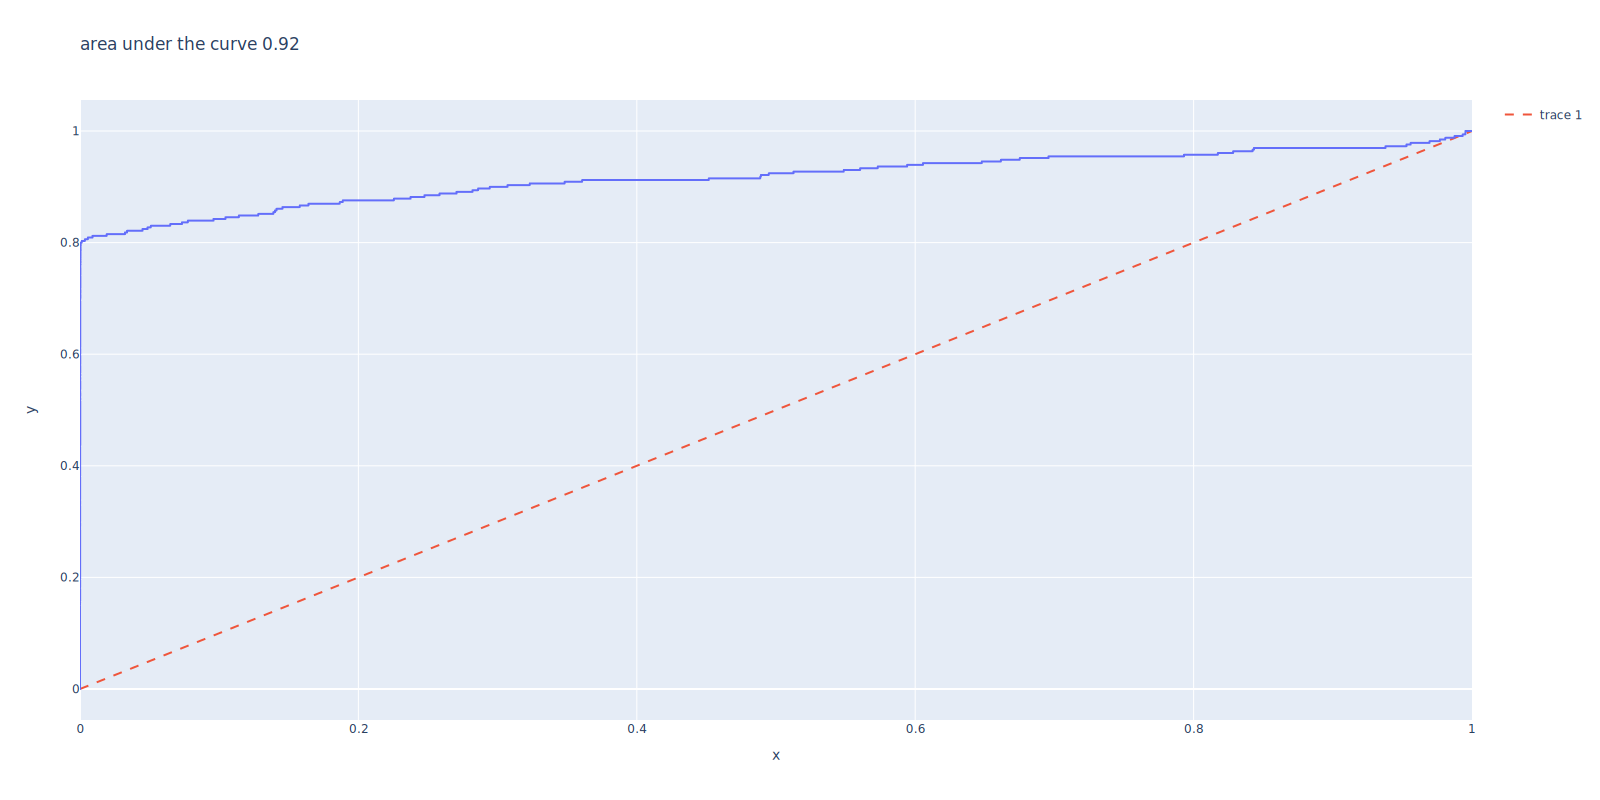
\includegraphics{mymarkdownfile_files/mymarkdownfile_45_0.svg}
\caption{svg}
\end{figure}

\begin{itemize}
\tightlist
\item
  This results is impressive considering its a unsupervised model we
  managed to etect 261 out of 330 fraudulent transactions.
\end{itemize}

\hypertarget{lets-test-our-model-on-test-data-and-look-at-the-precisionrecall-curve-and-roc-auc-curve.}{%
\subsection{Lets test our model on test data and look at the
precision/recall curve and roc-auc
curve.}\label{lets-test-our-model-on-test-data-and-look-at-the-precisionrecall-curve-and-roc-auc-curve.}}

\begin{itemize}
\tightlist
\item
  the below results are impressive again as we are able to capture
  almost 80\% of Fraud with 70\% precision and Area under the curve is
  .94.
\end{itemize}

\begin{Shaded}
\begin{Highlighting}[]
\NormalTok{preds}\OperatorTok{=}\NormalTok{ pd.concat([y\_test, pipe.predict\_proba(X\_test)], axis}\OperatorTok{=}\DecValTok{1}\NormalTok{)}
\NormalTok{preds.columns }\OperatorTok{=}\NormalTok{ [}\StringTok{\textquotesingle{}trueLabel\textquotesingle{}}\NormalTok{, }\StringTok{\textquotesingle{}anomalyScore\textquotesingle{}}\NormalTok{]}
\NormalTok{preds}
\end{Highlighting}
\end{Shaded}

trueLabel

anomalyScore

67353

0

7.976897e-07

67626

0

6.286458e-06

169699

0

1.170964e-05

217315

0

1.436673e-05

111420

0

3.173962e-05

\ldots{}

\ldots{}

\ldots{}

70762

0

5.631365e-06

69843

0

3.381275e-04

191806

0

2.466397e-04

259722

0

1.079170e-06

36616

0

1.314993e-06

93987 rows × 2 columns

\begin{Shaded}
\begin{Highlighting}[]
\NormalTok{precision, recall, thresholds }\OperatorTok{=}\NormalTok{  precision\_recall\_curve(preds[}\StringTok{\textquotesingle{}trueLabel\textquotesingle{}}\NormalTok{],preds[}\StringTok{\textquotesingle{}anomalyScore\textquotesingle{}}\NormalTok{])}
\NormalTok{average\_precision }\OperatorTok{=}\NormalTok{  average\_precision\_score(preds[}\StringTok{\textquotesingle{}trueLabel\textquotesingle{}}\NormalTok{],preds[}\StringTok{\textquotesingle{}anomalyScore\textquotesingle{}}\NormalTok{]).}\BuiltInTok{round}\NormalTok{(}\DecValTok{3}\NormalTok{)}
\NormalTok{px.scatter( x}\OperatorTok{=}\NormalTok{recall, y}\OperatorTok{=}\NormalTok{ precision, render\_mode}\OperatorTok{=}\StringTok{\textquotesingle{}webgl\textquotesingle{}}\NormalTok{, title}\OperatorTok{=}\NormalTok{average\_precision, width}\OperatorTok{=} \DecValTok{1600}\NormalTok{, height }\OperatorTok{=}\DecValTok{800}\NormalTok{).show(}\StringTok{"png"}\NormalTok{)}
\end{Highlighting}
\end{Shaded}

\begin{figure}
\centering
\includegraphics{mymarkdownfile_files/mymarkdownfile_49_0.png}
\caption{png}
\end{figure}

\begin{Shaded}
\begin{Highlighting}[]
\NormalTok{fpr,tpr,thresholds }\OperatorTok{=}\NormalTok{ roc\_curve(preds[}\StringTok{\textquotesingle{}trueLabel\textquotesingle{}}\NormalTok{], preds[}\StringTok{\textquotesingle{}anomalyScore\textquotesingle{}}\NormalTok{])}
\NormalTok{areaUnderROC }\OperatorTok{=}\NormalTok{ auc(fpr, tpr)}
\end{Highlighting}
\end{Shaded}

\begin{Shaded}
\begin{Highlighting}[]
\NormalTok{(}
\NormalTok{    px.line(x}\OperatorTok{=}\NormalTok{fpr, y}\OperatorTok{=}\NormalTok{tpr, title }\OperatorTok{=} \SpecialStringTok{f\textquotesingle{}area under the curve }\SpecialCharTok{\{}\BuiltInTok{round}\NormalTok{(areaUnderROC,}\DecValTok{2}\NormalTok{)}\SpecialCharTok{\}}\SpecialStringTok{\textquotesingle{}}\NormalTok{, width}\OperatorTok{=}\DecValTok{1600}\NormalTok{, height}\OperatorTok{=} \DecValTok{800}\NormalTok{)}
\NormalTok{    .add\_scatter(y}\OperatorTok{=}\NormalTok{[}\DecValTok{0}\NormalTok{,}\DecValTok{1}\NormalTok{], mode}\OperatorTok{=}\StringTok{"lines"}\NormalTok{, line\_dash}\OperatorTok{=} \StringTok{"dash"}\NormalTok{)    }
\NormalTok{    .show(}\StringTok{"svg"}\NormalTok{)}
\NormalTok{)}
\end{Highlighting}
\end{Shaded}

\begin{figure}
\centering
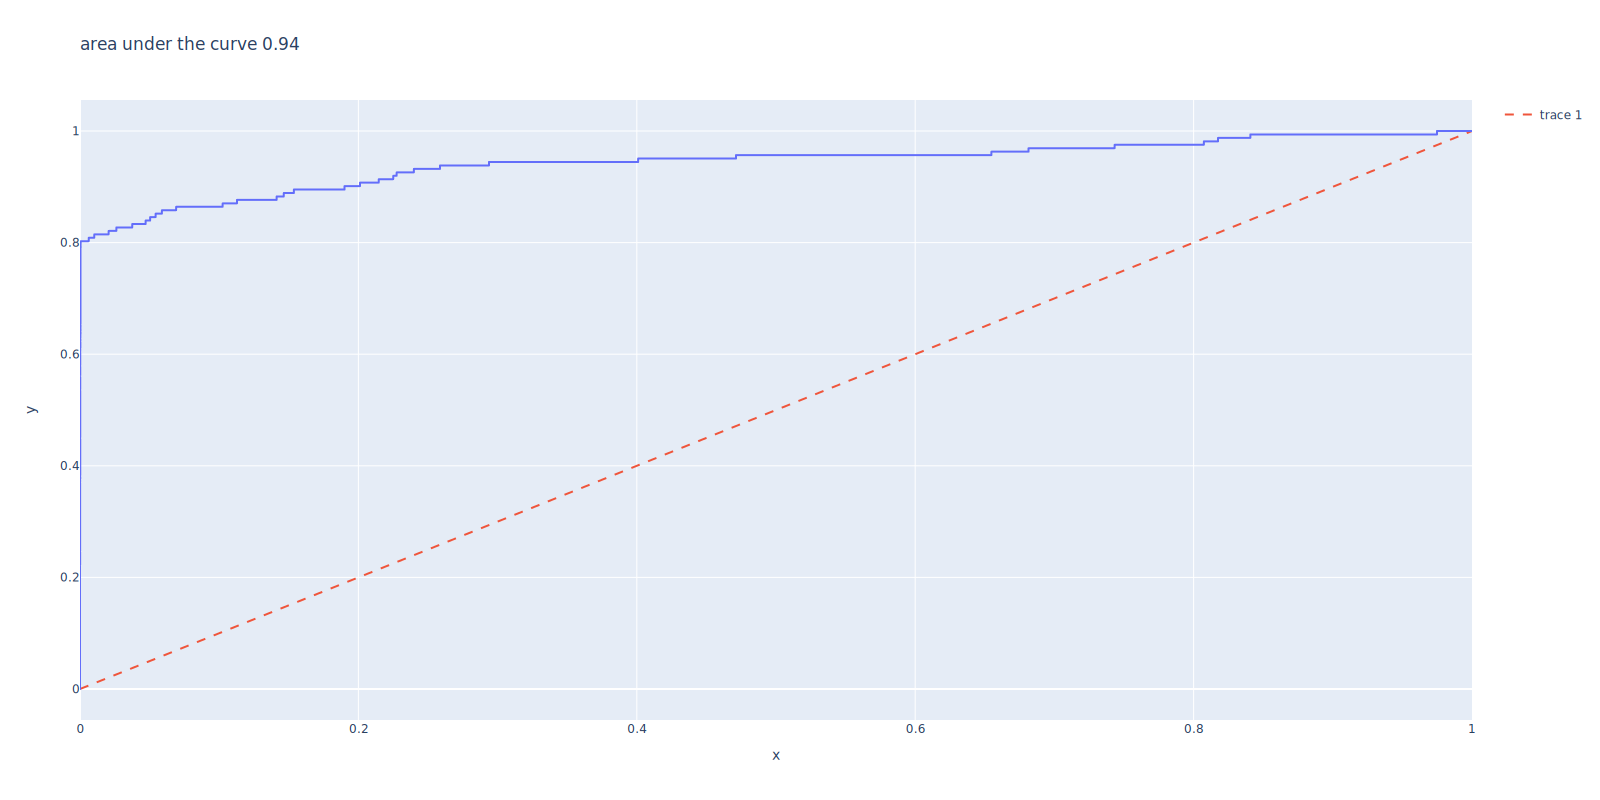
\includegraphics{mymarkdownfile_files/mymarkdownfile_51_0.svg}
\caption{svg}
\end{figure}

\# Conclusion:

\begin{Shaded}
\begin{Highlighting}[]
\ImportTok{import}\NormalTok{ pandas }\ImportTok{as}\NormalTok{ pd}
\ImportTok{import}\NormalTok{ numpy }\ImportTok{as}\NormalTok{ np}
\ImportTok{from}\NormalTok{ sklearn.datasets }\ImportTok{import}\NormalTok{ make\_classification}
\ImportTok{from}\NormalTok{ sklearn.linear\_model }\ImportTok{import}\NormalTok{ LogisticRegression}
\ImportTok{from}\NormalTok{ sklearn.metrics }\ImportTok{import}\NormalTok{ roc\_auc\_score ,roc\_curve}
\ImportTok{import}\NormalTok{ matplotlib.pyplot }\ImportTok{as}\NormalTok{ plt}
\ImportTok{from}\NormalTok{ sklearn.model\_selection }\ImportTok{import}\NormalTok{ train\_test\_split}


\CommentTok{\# generate a random dataset}
\NormalTok{X, y }\OperatorTok{=}\NormalTok{ make\_classification(n\_samples}\OperatorTok{=}\DecValTok{1000}\NormalTok{, n\_classes}\OperatorTok{=}\DecValTok{2}\NormalTok{, n\_features}\OperatorTok{=}\DecValTok{5}\NormalTok{,}
\NormalTok{                            n\_informative}\OperatorTok{=}\DecValTok{3}\NormalTok{, n\_redundant}\OperatorTok{=}\DecValTok{1}\NormalTok{, random\_state}\OperatorTok{=}\DecValTok{42}\NormalTok{)}

\CommentTok{\# split the data into training and testing sets}
\NormalTok{X\_train, X\_test, y\_train, y\_test }\OperatorTok{=}\NormalTok{ train\_test\_split(X, y, test\_size}\OperatorTok{=}\FloatTok{0.2}\NormalTok{, random\_state}\OperatorTok{=}\DecValTok{42}\NormalTok{)}

\CommentTok{\# fit a logistic regression model}
\NormalTok{clf }\OperatorTok{=}\NormalTok{ LogisticRegression(random\_state}\OperatorTok{=}\DecValTok{42}\NormalTok{)}
\NormalTok{clf.fit(X\_train, y\_train)}

\end{Highlighting}
\end{Shaded}

\hypertarget{sk-container-id-1}{}
In a Jupyter environment, please rerun this cell to show the HTML
representation or trust the notebook. On GitHub, the HTML representation
is unable to render, please try loading this page with nbviewer.org.

LogisticRegression

\begin{Shaded}
\begin{Highlighting}[]
\CommentTok{\# predict probabilities on the test set}
\NormalTok{probs }\OperatorTok{=}\NormalTok{ clf.predict\_proba(X\_test)[:, }\DecValTok{1}\NormalTok{]}

\CommentTok{\# calculate the roc\_auc score}
\NormalTok{auc }\OperatorTok{=}\NormalTok{ roc\_auc\_score(y\_test, probs)}

\CommentTok{\# plot the roc curve}
\NormalTok{fpr, tpr, thresholds }\OperatorTok{=}\NormalTok{ roc\_curve(y\_test, probs)}
\NormalTok{plt.plot(fpr, tpr, label}\OperatorTok{=}\StringTok{\textquotesingle{}ROC curve (area = }\SpecialCharTok{\%0.2f}\StringTok{)\textquotesingle{}} \OperatorTok{\%}\NormalTok{ auc)}
\NormalTok{plt.plot([}\DecValTok{0}\NormalTok{, }\DecValTok{1}\NormalTok{], [}\DecValTok{0}\NormalTok{, }\DecValTok{1}\NormalTok{], }\StringTok{\textquotesingle{}k{-}{-}\textquotesingle{}}\NormalTok{)}
\NormalTok{plt.xlabel(}\StringTok{\textquotesingle{}False Positive Rate\textquotesingle{}}\NormalTok{)}
\NormalTok{plt.ylabel(}\StringTok{\textquotesingle{}True Positive Rate\textquotesingle{}}\NormalTok{)}
\NormalTok{plt.title(}\StringTok{\textquotesingle{}Receiver operating characteristic example\textquotesingle{}}\NormalTok{)}
\NormalTok{plt.legend(loc}\OperatorTok{=}\StringTok{"lower right"}\NormalTok{)}

\CommentTok{\# find the optimal threshold}
\NormalTok{optimal\_idx }\OperatorTok{=}\NormalTok{ np.argmax(tpr }\OperatorTok{{-}}\NormalTok{ fpr)}
\NormalTok{optimal\_threshold }\OperatorTok{=}\NormalTok{ thresholds[optimal\_idx]}

\CommentTok{\# create a data frame with the test set predictions and probabilities}
\NormalTok{df }\OperatorTok{=}\NormalTok{ pd.DataFrame(\{}\StringTok{\textquotesingle{}actual\textquotesingle{}}\NormalTok{: y\_test, }\StringTok{\textquotesingle{}prob\textquotesingle{}}\NormalTok{: probs\})}

\CommentTok{\# assign a label of 1 or 0 based on the optimal threshold}
\NormalTok{df[}\StringTok{\textquotesingle{}pred\textquotesingle{}}\NormalTok{] }\OperatorTok{=}\NormalTok{ df[}\StringTok{\textquotesingle{}prob\textquotesingle{}}\NormalTok{].}\BuiltInTok{apply}\NormalTok{(}\KeywordTok{lambda}\NormalTok{ x: }\DecValTok{1} \ControlFlowTok{if}\NormalTok{ x }\OperatorTok{\textgreater{}=}\NormalTok{ optimal\_threshold }\ControlFlowTok{else} \DecValTok{0}\NormalTok{)}

\CommentTok{\# show the confusion matrix for the optimal threshold}
\NormalTok{confusion\_matrix }\OperatorTok{=}\NormalTok{ pd.crosstab(df[}\StringTok{\textquotesingle{}actual\textquotesingle{}}\NormalTok{], df[}\StringTok{\textquotesingle{}pred\textquotesingle{}}\NormalTok{], rownames}\OperatorTok{=}\NormalTok{[}\StringTok{\textquotesingle{}Actual\textquotesingle{}}\NormalTok{], colnames}\OperatorTok{=}\NormalTok{[}\StringTok{\textquotesingle{}Predicted\textquotesingle{}}\NormalTok{])}
\BuiltInTok{print}\NormalTok{(confusion\_matrix)}
\end{Highlighting}
\end{Shaded}


\end{document}
